%%%%%%%%%%%%%%%%%%%%%%%%%%%%%%%%%%%%%%%%%
%
% (c) 2018 by Jennifer Laaser
%
% This work is licensed under the Creative Commons Attribution-NonCommercial-ShareAlike 4.0 International License. To view a copy of this license, visit http://creativecommons.org/licenses/by-nc-sa/4.0/ or send a letter to Creative Commons, PO Box 1866, Mountain View, CA 94042, USA.
%
% The current source for these materials is accessible on Github: https://github.com/jlaaser/pogil-polymers
%
%%%%%%%%%%%%%%%%%%%%%%%%%%%%%%%%%%%%%%%%%

\renewcommand{\figpath}{content/intro/nomenclature/figs}
\renewcommand{\labelbase}{nomenclature}

\begin{activity}[Molecular Weight Distributions in Step-Growth Polymerizations]

\begin{instructornotes}

	This activity introduces students to key concepts related to the nomenclature of polymers.
	
	After completing this activity, students will be able to:
			\begin{enumerate}
				\item \dots
			\end{enumerate}
			
	\subsection*{Activity summary:}
	\begin{itemize}
		\item \textbf{Activity type:} Learning Cycle
		\item \textbf{Content goals:} Nomenclature of polymers
		\item \textbf{Process goals:} %https://pogil.org/uploads/attachments/cj54b5yts006cklx4hh758htf-process-skills-official-pogil-list-2015-original.pdf
			written communication, critical thinking, information processing
		\item \textbf{Duration:} TBD
		\item \textbf{Instructor preparation required:} none beyond knowledge of relevant content
		\item \textbf{Related textbook chapters:}
			\begin{itemize}
				\item \emph{Polymer Chemistry} (Hiemenz \& Lodge): sections 1.3, 1.5, and 1.6
			\end{itemize}
		%\item \textbf{Facilitation notes:}
		%	\begin{itemize}
		%		\item \dots
		%	\end{itemize}
	\end{itemize}

\end{instructornotes}

	%\textbf{Focus question:} Put a central question for the students to consider through this exercise here.

\begin{model}[ABC]

	Here is the first model for students to consider

	Here is a second paragraph of text, followed by an image:

	% to include images, put them in the folder specified by figpath and then use:
	\centerline{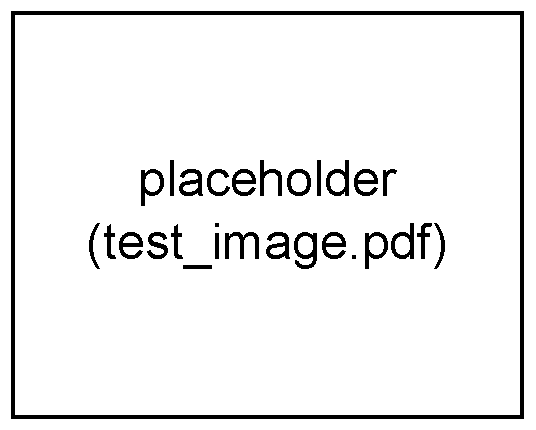
\includegraphics[width=0.5\textwidth]{\figpath/test_image.pdf}}

\end{model}


\begin{ctqs}

	\question First question?
	
		\begin{solution}[1in]
		\end{solution}
		
	\question Second question?
	
		\begin{solution}[1in]
			Here is a dummy answer in the solution space.
		\end{solution}
		
	\question Third question?
	
		\begin{solution}[1in]
		
			\studentdisplay{Here is something we show only when we process the student version.}
			
			\instructordisplay{Here is something we show only when we process the instructor version.}
			
		\end{solution}

\end{ctqs}



\begin{model}[DEF]

	Here is a second model for students to consider.

\end{model}

\begin{ctqs}

	\question First question?
	
		\begin{solution}
		\end{solution}
	
	\question Second question?
	
		\begin{solution}
		
			Here's a solution environment that doesn't have a height set, but does have content.
			
			(The previous solution environment has no height and no content.)		
		
		\end{solution}
\end{ctqs}

		
\begin{infobox}
	Here is some useful information that might help the students with the next few critical thinking questions.
	In some cases, it might include an equation:
	\begin{equation*}
		a^2 + b^2 = c^2
	\end{equation*}
	or even more than one equation:
	\begin{equation*}
		x=\frac{-b \pm \sqrt{b^2-4ac}}{2a}
	\end{equation*}
\end{infobox}

\begin{ctqs}

	\question First question?
		\begin{solution}[1in]
		\end{solution}
	
	\question Second question?
		\begin{solution}[1in]
		\end{solution}
\end{ctqs}



\begin{exercises}

	\exercise First exercise ~\answer{a short answer}
	\exercise Second exercise
	
\end{exercises}


\begin{problems}

	\problem First exercise
	\problem Second exercise
	
\end{problems}


	
\end{activity}